\subsection{Présentation de l'approche à composants}
    
Le terme «~composant~», défini dans l'approche de l'ingénierie du logiciel basée sur les composants (\emph{Component-Based Software Engineering -- CBSE}) étant très générique, en donner une définition exacte et précise paraît difficile car cela dépend fortement du contexte de son utilisation. Cependant on peut se baser sur des définitions faites dans la littérature :

\begin{quote}
  \emph{ A software component is a unit of composition with contractually specified interfaces and explicit context dependencies only. A software component can be deployed independently and is subject to composition by third parties.} \cite{Szyperski:2002:CSB:515228}
\end{quote}
  
\begin{quote}
  \emph{ A component is a nontrivial, nearly independent, and replaceable part of a system that fulfills a clear function in the context of a well-defined architecture. A component conforms to and provides the physical realization of a set of interfaces.} \cite{kruchten1998modeling}
\end{quote}
  
\begin{quote}
  \emph{ A component is a unit of distributed program structure that encapsulates its implementation behind a strict interface comprised of services provided by the component to other components in the system and services required by the component and implemented elsewhere. The explicit declaration of a component's requirements increases reuse by decoupling components from their operating environment.} \cite{DBLP:conf/cds/PryceC98}
\end{quote}
  
Ces différentes définitions permettent de faire ressortir des notions qui se retrouvent dans la plupart des approches à composants : 
    
\begin{description} 

  \item[interfaces] C. Szyperski définit une interface d'un composant comme étant un point d'accès au service du composant \cite{szyperski1999components} permettant de décrire comment les composants peuvent être assemblés ou utilisés dans une architecture. On parle d'interfaces << requises >>, les interfaces permettant de décrire les besoins d'un composant et d'interfaces << fournies >>, les interfaces permettant de définir les fonctionnalités que proposent le composant aux autres composants.
  
  \item[indépendance] Il faut voir un composant comme un élément indépendant de tout système. Il doit être assez générique pour pouvoir se connecter à d'autres composants au sein d'une nouvelle application en fournissant un ensemble de services, sans être trop spécifique à un système. 
  
  \item[architecture] La notion d'architecture permet de représenter le plan de l'application et permet de décrire comment l'application doit être conçue afin de respecter les spécifications mises en place.
  
  \item[composition] Le mécanisme de composition permet de créer à partir d'un assemblage de composants, un nouveau composant plus complexe, en encapsulant des composants afin de pouvoir réutiliser directement cet assemblage. Ce nouveau composant est dit composite car constitué de composants qui deviennent des sous-composants (composants interne), pouvant être eux aussi des composants composites ou des composants primitifs \footnote{un composant est dit primitif s'il ne contient pas de sous-composants}.
  
  \item[service] Les services permettent de représenter la logique métier d'un composant. Géné\-ralement présents uniquement dans des composants primitifs, certaines approches essaient de définir des services pour des composants composites. 
  
\end{description}
    
\subsection{Les principes du développement par composants}

  De nombreux concepts permettent la réutilisabilité dans le développement (appel de fonction, importation de module, héritage entre classes, paramétrage de framework, assemblage de composants, etc.). Cependant, même si ces différentes techniques permettant de mettre en avant cette notion de réutilisabilité, les composants ont fait de la réutilisation le fer de lance de leur approche.\\\par  
    
  On identifie deux acteurs dans le développement par composants \cite{fabresse2007decoupage} : le dévelop\-peur de composants et l’architecte d’application (cf figure \ref{fig:reusecomponent}). Le rôle du développeur va consister à réaliser des composants indépendants. L'architecte récupère les composants déjà créés par un développeur et réalise une intégration dans son assemblage de composants existant. Il est bien sûr possible pour une personne d'avoir les deux rôles à la fois, mais il est important dans ce paradigme de rendre son composant indépendant de l'application. \\\par 
      
\begin{figure}[!t]
\centering
\scalebox{.5}{
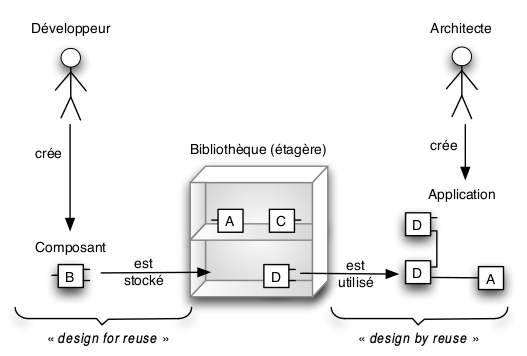
\includegraphics{images/reuse.png}
}
\caption{Vision simplifiée du processus de développement par composants, extrait de \cite{fabresse2007decoupage}}
\label{fig:reusecomponent}
\end{figure}
  
  Nous avons vu que l'architecture logicielle permettait de définir comment notre application devait être construite. C'est pour cela que nous avons besoin de visibilité sur cette architecture afin de bien appréhender comment notre application est réalisée et de visualiser toutes les intéractions entre les éléments de l'application, permettant ainsi de vérifier que cette architecture respecte bien les spécifications. Dans le développement par objets, la notion d'architecture est utilisée lors de la phase de conception de l'application. Le développeur peut se faire aider par des outils de représentation graphique, comme UML, mais cette représentation n'est que peu maintenue lors de la phase d'implémentation. Les modifications apportées par celle-ci ne sont plus visibles et donc n'assure plus que l'architecture obtenue soit conforme aux spécifications. \\\par
  
  Le développement par composants arrive à corriger cela, en rendant explicite cette visibilité sur l'architecture, soit à la manière des ADLs (Architecture Description Languages), qui permettent de décrire la structure et de définir le comportement des composants à travers leurs assemblages, par une représentation abstraite, soit directement dans l'implémentation des composants par l'approche des langages à composants, qui définissent l'architecture au sein même des composants. Par conséquent, même si pendant la phase d'implémentation on décide de modifier l'architecture de nos composants, on ne perdra pas la visibilité sur l'architecture de notre application car elle est écrite explicitement. \\\par
  
\subsection{Les grandes familles du développement à base de composants}
      
      \subsubsection{Les approches des génératives}
      
      Les approches des génératives se situent à un haut niveau d'abstraction afin de modéliser et gérer des systèmes logiciels complexes. Cette représentation se base généralement sur les ADLs, permettant de décrire les architectures à base de composants en y décrivant leurs comportements, leurs intéractions avec les autres composants et leurs configurations ainsi que leurs besoins explicites. La stratégie de cette approche générative consiste donc en la modélisation d'une architecture de composants << initiale >> décrite de manière formelle. Ensuite un << squelette >> d'application dans un langage de programmation précis qui respectera les spécifications du système est généré à partir de l'architecture. Cette représentation étant abstraite, elle est indépendante des langages de programmation qui implémentent les composants, permettant ainsi de s'adapter à tous types de plateformes. \\\par
      
      Parmi les modèles les plus importants dans cette famille, nous retrouvons UML et Fractal. \\\par
      
          \textbf{UML -- un langage de modélisation graphique pour composants}
      
      UML (Unified Modeling Language) est un langage de modélisation graphique standardisé par l'OMG (\emph{Objet management groupe}) \footnote{http://www.omg.org/spec/UML}. Dans sa première version, UML intègre déjà la notion de composant, comme étant une entité indépendante et communiquant avec d'autres composants au travers d'interfaces. La version 2.0 d'UML \cite{specificationuml} a permis d'améliorer cette vision des composants, en s'inspirant aussi des mécanismes et concepts des ADLs, introduisant la notion de port, de connecteur et de composant composite.

Un composant UML est donc une entité autonome, qui communique avec les autres composants de l'architecture au travers d'interfaces, regroupées dans des ports qui expriment des rôles. Un composant peut disposer de plusieurs ports, où un port regroupe un ensemble d'interfaces requises ou fournies. Le port permet donc de réaliser un point de communication entre l'environnement extérieur du composant et son architecture interne. 
      
 Cette connexion entre composants est permise par la notion de connecteur, qui permet de représenter les possibilités de communication entre les composants. Il existe deux types de connecteurs : d’assemblage et de délégation. Un connecteur d'assemblage permet de lier deux interfaces de deux composants. Avec une interface requise pour notre premier composant et une interface fournie pour notre deuxième composant. Cette connexion ne peut se faire que si les deux interfaces ont la même signature. Un connecteur de délégation quant à lui est utilisé afin de réaliser une connexion entre ses interfaces ou ports vers les interfaces ou ports de ses composants internes, permettant ainsi une délégation d'un besoin ou d'un service vers un composant interne.
        
    UML apporte cet aspect visuel à la représentation des architectures à composants qui manquent aux autres approches, aidant ainsi un architecte à mieux visualiser l'architecture qu'il est en train de construire. Par contre, il ne permet pas de réaliser l'implémentation et la manipulation de composants sans les coupler à une autre technique. \\\par 
    
        \textbf{Fractal -- un framework à composants intégrant un ADL}
        
        Fractal \cite{DBLP:journals/spe/BrunetonCLQS06} est une spécification d'un modèle à composants proposé par le consortium \emph{ObjectWeb} en 2002. Il propose un framework pour la création d'applications déployables sur un serveur, ainsi que la création et la manipulation de composants, intégrant en plus un ADL pour la description de l'architecture des composants. Il met en avant le concept de composant composite, de composant partagé, un mécanisme d'introspection et la possibilité de configuration dynamique. 
        
        Un composant Fractal est composé de deux parties. La partie \emph{contenu} qui est consti\-tuée des fonctionnalités que propose le composant, en étant soit un composant primitif qui dans son \emph{contenu} va implémenter la logique métier, soit un composant composite qui encapsule un assemblage de composants qui réalise les fonctionnalités attendues. La deuxième partie d'un composant est appelé la \emph{membrane}, qui contient les parties non-fonctionnelles du composant, intégrant les différentes interfaces qui communiquent avec le monde extérieur, ainsi que les interfaces qui permettent le contrôle du composant. Parmi les modèles les plus importants dans cette famille, nous retrouvons UML et Fractal. \\\par
        
        Une interface a deux types de visibilité : externe qui est visible depuis l’extérieur du composant et permettra une liaison avec d'autre composants et interne permettant une liaison avec son contenu. Une interface peut avoir différents rôles :
        
        \begin{enumerate}
        
          \item Le rôle de serveur, qui est une interface fournie proposant les différents services du composant
          
          \item Le rôle de cliente, qui est une interface requise représentant les besoins du composant
          
          \item Le rôle de contrôle, permettant la configuration dynamique du composants avec la possibilité de modifier ces liaisons avec les composants externe, de modifier son assemblage interne (modification des liaisons internes) et la gestion du cycle de vie du composant
        
        \end{enumerate}
        
        Afin de pouvoir connecter des composants entre eux, il faut connecter une interface de l'un avec une interface de l'autre. Cette connexion est appelée liaison (\emph{binding}) et peut être de trois types : une liaison normale (\emph{normal binding}) entre une interface serveur externe d'un composant et une interface cliente externe d'un autre composant, une liaison d'export (\emph{export binding}) entre une interface cliente d'un composite et une interface serveur d'un composant interne, permettant donc la délégation d'un service fourni par notre composant composite qui sera fourni par son composant interne, et une liaison d'import (\emph{import binding}) entre une interface serveur interne d'un composant composite et une interface cliente externe d'un composant interne permettant la délégation d'un besoin de notre composant interne au composant composite.
        
        Étant un modèle abstrait, il permet de s'abstraire de tous langages et de plateformes pour la gestion de composants. Différentes implémentations ont été réalisées (par exemple en Java avec Julia ou en C++ avec Cecilia). En effet l'ADL qu’intègre Fractal est décrit dans une syntaxe XML et spécifié de manière indépendante des langages de programmation. Les différentes implémentations proposent cependant un mécanisme de génération de code à partir de l'ADL pour réaliser l'implémentation des composants. \\\par

    \subsubsection{La famille des frameworks}     
   
    La famille des frameworks à composants utilise les langages de programmation à objets connus, pour la création et la manipulation de composants afin de modéliser un système. Cette approche permet au développeur d'utiliser les composants afin de bien séparer les besoins fonctionnels et les besoins non-fonctionnels. Principalement utilisé dans le monde professionnel, les frameworks à composants proposent aux développeurs de créer, déployer et configurer une application.  \\\par
    
    Parmi les frameworks les plus importants dans cette famille, nous retrouvons Enterprise JavaBeans et Spring. \\\par
    
    \textbf{Enterprise JavaBeans -- un framework à composants pour la création d'applications distribuées} 
    
    L'approche de composant mise en place par Enterprise JavaBeans (EJB), développée au sein de la plateforme Java Enterprise Edition (JEE), propose un modèle à composants serveur permettant la réalisation d'applications distribuées \cite{specificationejb}.
    
    Un composant EJB s’exécute dans un conteneur au sein d'un serveur JEE. Les conteneurs gèrent les instances des EJB, tandis que le serveur fournit au conteneur des besoins non-fonctionnels.
    
    Un composants EJB est regroupé en trois catégories : session, entité et message. Une instance d'un composant entité permet de représenter un concept métier, ayant pour but de représenter des données pouvant être stockées dans une base de données. Une instance d'un composant message permet la gestion de messages asynchrones reçus par le serveur depuis le client. Une instance d'un composant session permet de fournir des services définis par des méthodes, pouvant être sans état (stateless) ou avec état (stateful).
    
    Un composant EJB communique ses services par une interface \emph{remote}, spécifiant ainsi les méthodes que fournit une instance d'un EJB au monde extérieur. Il permet sa configuration et la gestion de son cycle de vie par une interface \emph{home} qui est fournie par son conteneur. Cependant on ne peut définir le besoin d'un EJB au moyen d'une interface requise. Les propriétés d'un EJB sont définies dans un descripteur de déploiement permettant au conteneur EJB de savoir comment gérer les composants pendant leur exécution.
    
    L’approche des EJB ne permet pas la réalisation de composant composite. Ainsi une architecture sera dite << à plat >>, chaque composant sera au même niveau que les autres, permettant une vision horizontale de l'architecture. Mais cela peut s’avérer répétitif de réaliser l'ensemble de toutes les différentes connexions entre composants sans pouvoir utiliser la composition pour réutiliser un assemblage de composants. \\\par
    
    \textbf{Spring -- un framework à composants pour la création d'applications modulaires}
    
    Spring \footnote{https://spring.io/} est un framework utilisé afin de fournir une infrastructure compréhensive pour la création d'applications Java. Comme la grande majorité des frameworks, il fonctionne sur le principe de l'inversion de contrôle (IoC -- patron de conception où le processus d’exécution d'une application est géré par le framework), qui est assurée par la recherche de dépendances et l'injection de dépendances automatique, tout en offrant un ensemble de fonctionnalités facilitant l'accès aux données, le développement web, les tests automatisés, etc., qui sont organisés en modules.  
    
    Un module est une unité de code indépendante d'un système logiciel. Il possède deux caractéristiques fondamentales~:  une forte cohésion (le module se focalise sur une tâche unique), et un couplage minimal (le module a de faibles dépendances avec les autres modules). Un module est décrit par une spécification, qui définit les signatures des fonctions publiques fournies par le module et une implémentation, qui implémente les fonctions fournies. Il permet de répondre aux problématiques de maintenabilité, réutilisabilité et testabilité. 
    
    Le cœur de Spring est géré par le \emph{Spring Core Container}, qui est un ensemble de modules permettant la réalisation du conteneur Spring de l'application, qui a un comportement similaire au conteneur EJB. Il implémente l'IoC et permet de gérer la création, le cycle de vie et les dépendances des \emph{bean} qu'il contient (un composant Spring (bean) étant une classe Java qui implémente une ou plusieurs interfaces fournies). La description des beans est principalement décrite dans des fichiers XML mais peut se faire dans le code source avec l'utilisation d'annotations Java ou l'utilisation de code source de manière spécifique par le framework.
    
    Cette description décrit la classe du bean, ainsi que son identifiant. On peut injecter à cette description des constructeurs, avec comme argument des valeurs primitives ou des références vers d'autre beans (grâce à par leur identifiant). On peut aussi rajouter un ensemble de propriétés (i.e. attribut privé ayant un getter et un setter), définis par un nom et une valeur d'un type primitif ou une référence vers un autre bean. La reconfiguration d'un bean (par exemple, modifier la référence vers un bean d'une propriété), se réalise par la modification textuelle de la référence et la relance de l'exécution de l'application. Un bean composite est obtenu par la déclaration d'un bean interne (inner bean), qui se comporte comme une classe interne. \\\par 
             
    \subsubsection{La famille des langages à composants}
    
    \label{sec:presentcomponent}
    
    L'approche des langages à composants s'articule autour d'un seul langage de programmation pour permettre de définir une architecture de composants et l'implémen\-ta\-tion de ses composants. Ce regroupement de ses deux principes permet de faciliter le développement, car le programmeur ne doit connaître qu'un seul langage.  
    Cette approche autour d'un seul langage permet de ne pas avoir de violation de contraintes architecturales, qui pouvait se produire avec les ADLs, qui ont une description dans un langage et l'implémentation dans un autre.\\\par 
    
    Parmi les langages à composants les plus importants dans cette famille, nous retrouvons ArchJava et ComponentJ. \\\par
    
      \textbf{ArchJava -- un langage à composants} 
      
      ArchJava \footnote{http://www.archjava.org/} créé en 2001 \cite{DBLP:conf/icse/AldrichCN02}, s'inspire de l'approche composant que proposent les ADLs pour la description d'architecture, tout en permettant l'implémentation de ces composants au sein d'un nouveau langage qui est une extension du langage Java.
      
      Un composant est dans ce monde un <<objet particulier>>, qui s'obtient par instanciation de la classe \texttt{component class}. Cette classe de composant permet de regrouper les informations du composant : ses ports, ses méthodes, ses attributs, ainsi que ma description de son assemblage interne à travers des connexions.
      
  Deux composants ne peuvent communiquer entre eux que s'ils sont explicitement connectés par la primitive \texttt{connect}. Cette primitive introduit la connexion entre composants par la liaison de leurs ports respectifs pour la première fois dans l'histoire des approches à composants 
  
 Un port définit une liste de méthodes fournies et requises, différenciées respectivement par les primitives \texttt{provides} et \texttt{requires}. Une méthode fournie permet d'introduire une fonctionnalité proposée par le composant au monde extérieur. Les autres composants n'ont accès à cette méthode que par le biais du port. Une méthode requise permet de décrire une fonctionnalité attendue par notre composant. Deux ports ne peuvent se lier entre eux que si les signatures des méthodes requises et fournies qu'ils définissent sont compatibles entre eux. \\\par 
  
  \textbf{ComponentJ -- un langage à composants} 

  ComponentJ \footnote{https://projectos.fct.unl.pt/projects/di-componentj/wiki} présenté par \cite{seco2008component}, propose un modèle à composants, explicitant les dépendances entre composants, la création dynamique de nouveaux composants, la reconfiguration au runtime et un typage fort pour les composants. Il ne faut pas le confondre avec son cousin ArchJava, qui comme lui est une extension du langage Java, car ils sont tous les deux conceptuellement différents.

  Par exemple, un composant est un élément instance d'une classe dans ArchJava, alors qu'un composant est un descripteur instanciable d'objets en ComponentJ. Ce descripteur permet de définir la structure et le comportement de chacune de leurs instances en décrivant les ports et en définissant les services fournis par les objets. En effet, un objet en ComponentJ est une instance de composant, qui a un comportement comparable à un objet Java. Cependant il doit être typé par une interface (\textbf{object interface}) qui définit l'ensemble des services que fournira notre objet, à travers la définition d'un seul port fourni.
    
  Les ports sont des interfaces (\textbf{port interface}) qui définissent un ensembles de signatures de méthodes. Ces méthodes représentent les services des composants et seront dites requises ou fournies en fonction du rôle du port qui les définit. En effet si un port a un rôle de fourni dans un composant alors ce composant devra implémenter ces méthodes, identifiées par la primitive \texttt{methods}. Tandis que si un port a un rôle de requis, alors le composants pourra invoquer ces méthodes afin de les utiliser. 
  
  Les configurateurs sont des blocs d'instructions présents dans les composants. Ils permettent le mécanisme de composition ou de connexion. Ils peuvent être utilisés pour la création au runtime de nouveaux composants, ainsi que la reconfiguration des comportements et la restructuration des composants.
  
  ComponentJ a fait le choix de mettre en avant l'assemblage de composants, qui ne sont pas ici des instances mais des descripteurs, leur instanciation étant possible uniquement si les dépendances requises sont satisfaites ce qui permet d'avoir une forte sûreté à l'exécution, mais rend plus contraignante l'utilisation des composants. En effet, un développeur doit satisfaire l'ensemble des besoins de chaque composant, même ceux qui seraient inutiles dans l'application. \\\par
  
  

    
      
